\section{Experiments}

\subsection{Dataset}
Currently, the largest labeled dataset for exoplanet detection problem is maintained by NASA, based on the effectiveness of Kepler mission. %\footnote{Kepler measured the light variation of thousand of distant stars in search of periodic planetary transit within our galaxy neighborhood.}. 
We use the \textit{Kepler Objects of Interest} (KOI) dataset\footnote{http://archive.stsci.edu/search\_fields.php?mission=kepler\_koi} provided by MAST (\textit{Mikulski Archive for Space Telescopes}) \citep{akeson2013nasa}, which is composed by 8054 records with the corresponding light curves. Every Kepler Object of Interest (KOI) is a region of interest in the sky that shows a periodic behavior based on thresholding events. 
These objects are categorized according to Nasa Exoplanet Science Institute\footnote{http://nexsci.caltech.edu/}, as \textit{Confirmed} (2281), claimed exoplanets through extensive scientific analysis and follow ups; \textit{False Positive} (3976), initially selected as candidate exoplanets but additional evidence show they are not; or \textit{Candidate} (1797), those that are still under study (unlabeled data).
%\begin{itemize}
%\item 2281 \textit{Confirmed}: those that through extensive science analysis have been confirmed as exoplanet.
%\item 3976 \textit{False Positive}: those that were initially selected as candidate exoplanets but additional evidence showed they are not. 
%\item 1797 \textit{Candidate}: those that are still under study (unlabeled data). 
%\end{itemize}
%According to MAST, between the reasons to label a candidate object as a \textit{False Positive} there are: i) the observation did not match with the star position on study, i.e. the transit was from another object (non-planetary) in the background, ii) the deep of the even transit was statistically different to the deep of the odd transits showing a binary system, i. e. two stars orbiting their barycenter. 
Almost all stars under study are ``new" stars that has not been studied before, or only some of them (around 25\%) has been previously studied in the search of extrasolar planets.


Multiple KOIs are obtained from each host star, and each object contains raw measurements (i.e., light curve, see Figure \ref{fig:curva_muestreo} for an example) with timestamps, including the instrumental error associated to each measure. 
Some important information regarding to the light curve is that the sampling rate of Kepler is 0.0204 BJD on average (i.e., half an hour), but there is a 22.98\% of missing values per light curve on average. Each light curve has approximately 55000 effective measurements (a collection period of 4 years).

\begin{figure}[t]
    \centering
    \begin{tabular}{cc}
    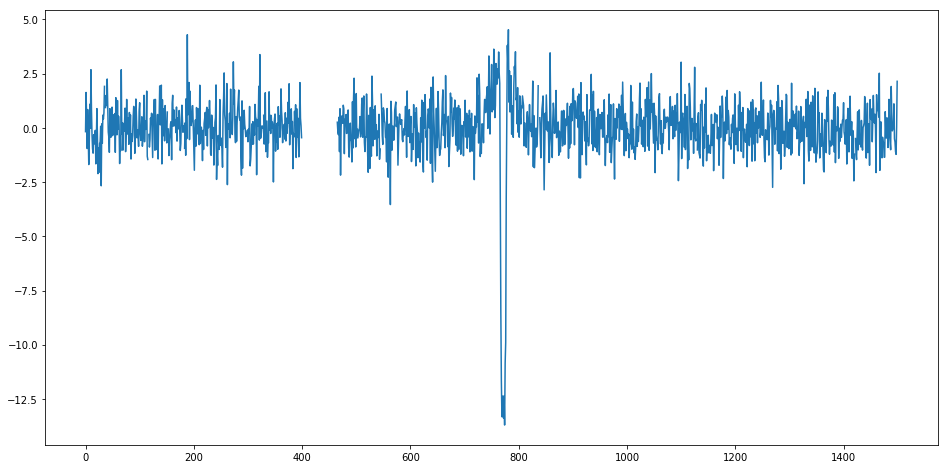
\includegraphics[width=0.45\linewidth]{imgs/curva1.png} &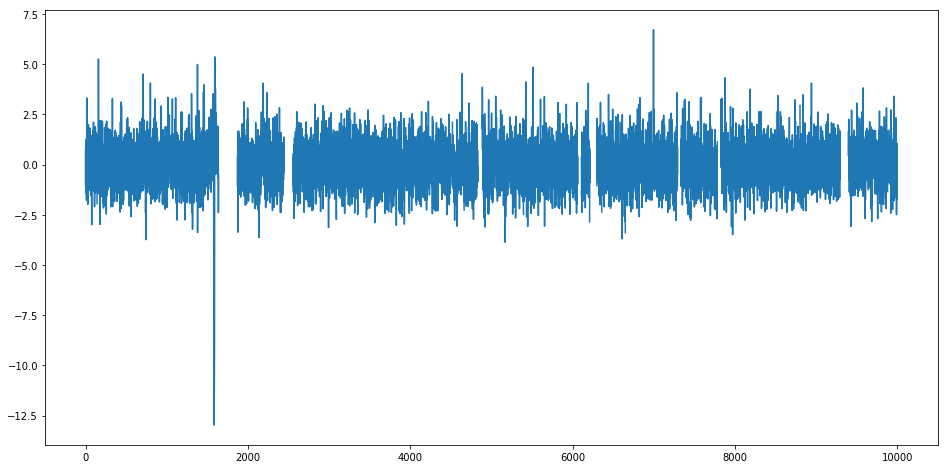
\includegraphics[width=0.45\linewidth]{imgs/curva2.png}  \\
         %&
    \end{tabular}
    \caption{Extracts of a a random light curve in the raw representation.}
    \label{fig:curva_muestreo}
\end{figure}

The archive also provides a set of metadata values, some of them (usually related to the star) are cross-matched from other catalogues. For comparing our self-generated features with model-based ones, we have selected only those that can be directly obtained from the light curves by following the best-fit parameter with a Mandel-Agol model \citep{mandel2002analytic}, these are\footnote{Documentation available at: \href{https://exoplanetarchive.ipac.caltech.edu/docs/API\_kepcandidate\_columns.html}{Kepler Objects of Interest -- NExScI}}: \textit{Period}, \textit{First Transit Time}, \textit{Inclination}, \textit{Planet Radius} (over Stellar Radius), \textit{Semi-major Axis} (over Stellar Radius), \textit{Limb Darkening Coefficients}, \textit{Transit Duration}, \textit{Impact Parameter} and \textit{Fitted Stellar Density}.

%\subsubsection{Metadata}
%From all the high-level features (metadata) that were available, we have selected the features that could be extracted only from the light curve\footnote{Documentation available at: \href{https://exoplanetarchive.ipac.caltech.edu/docs/API\_kepcandidate\_columns.html}{Kepler Objects of Interest -- NExScI}}, without cross-matching from other cataloges. Note that the first five features listed were calculated as one of the best-fit parameter per feature on a Mandel-Agol model \citep{mandel2002analytic}.
%\begin{itemize}
%\item \emph{Period}: the interval between consecutive planetary transits in days. 
%\item \emph{First Transit Time}: the time when the exoplanet pass in front of the host star in Barycentric Julian Date (BJD) .  
%\item \emph{Inclination}: the angle, in degrees, between the plane of the sky (perpendicular to the line of sight) and the orbital plane of the object\footnote{90 degrees is a orbit in the line of sight}.  
%\item \emph{Planet Radius} (over Stellar Radius): the inferred radius of the object.  
%\item \emph{Semi-major Axis} (over Stellar Radius): orbital radius based on the axis of an elliptic orbit.  
%\item \emph{Limb Darkening Coefficients}: models the light variation (darkening) on the edges of the star, two coefficient (linear and quadratic). To be sure, Kepler used cross-matching.
%\item \emph{Transit Duration}: time in days between first contact and last contact, i.e. eclipse duration. Calculated based on the transit period, planet radius and orbit radius.
%\item \emph{Impact Parameter}: distance between the object and the sight axis to the star. Calculated based on the orbit radius and the inclination.
%\item \emph{Fitted Stellar Density}: calculated based on a small planet approximation with the planet radius, transit period and duration.
%\end{itemize}


%\subsection{Pre-processing}
We use Kepler's detrended pipeline \citep{fanelli2011kepler} to obtain a standard light curve for our experiments.% That is, a representation that expresses the variations related to a local window behavior. 
It consists on applying a polynomial fit, Sav-Gol filter \citep{savitzky1964smoothing}, of two degrees with a window of 151 and subtract it to the light curve. Then, it subtracts a moving median filter with a window of 25. Finally, we remove positive outliers that are higher than $5\sigma$ and removes negative outliers lower than $40 \sigma$. 

We perform a random (80/20)\% split to create a training and validation set respectively. Also as a data augmentation step, we double the data by a mirror operation for each light curve \citep{tiensuu2019detecting}. This would represents that the same object, with the same properties, orbits the star in the opposite direction.
%otros trabajos que aumentan de esa manera: shallue, andsdell.

\subsection{Reference Methods}
As our main baselines we consider the specialized handcrafted features that are based on the scientific knowledge of the exoplanet problem. The metadata information on the Kepler mission described above is one of them. Another is the more general feature set proposed by \citep{cabral2018fats} called \emph{feets} (i.e, Feature Extractor for Time Series)\footnote{\texttt{https://feets.readthedocs.io}}. The \emph{feets} features can go from basic statistical measures like the maximum or the mean, to more complex time-series characteristics such as the autocorrelation function.

From the classical methods, we have selected the PCA feature extractor over the frequency domain representation of the time series (spectrum), which we named F-PCA proposed by \citet{bugueno2018refining}. The number of components to extract are selected over a validation set.

Finally, for comparing to a competitive deep learning method, we combine the proposals of \citet{aguirre2019deep} and \citep{shallue2018identifying} into a 1D CNN that uses the raw light-curve. On one hand, \citet{aguirre2019deep} use the time as an extra channel to the model in order to process unevenly-sampled time series, as are variable stars. On the other, \textit{Astronet} \citep{shallue2018identifying} processes the inputs with a deep 1-dimensional convolutional model obtaining state of the art results on transit detection with folded light curves. 

\subsection{Evaluation}
Since the exoplanet problem is an instance of unbalanced binary classification problem, we need to select quality measures beyond the standard accuracy. We use the \textit{F1-score} macro, that summaries \textit{precision} and \textit{recall} metrics in just one value equitably through the classes. \textit{F1-score} macro is defined as the harmonic mean between the two metrics previously mentioned, being high when both are. 

\subsection{Network Architecture}

\begin{table}[!t]
\centering
\caption{Deep Learning architecture models. At the left, the best 2D CNN model for MTF Images; At the right, the best 1D CNN model for 1D CNN raw method. All convolutional layers and 128-unit dense layer use \textit{relu} activation function, while the last dense layer use \textit{sigmoid}. As the 1D CNN model processes measurements and time separately, two flatten vectors are obtained. $k_s$ stand for kernel size. \vspace{0.1cm}}
\label{tab:model:arch}
\begin{tabular}{|cc|cc|} \hline
\multicolumn{2}{|c|}{\textbf{2D CNN MODEL}}    &    \multicolumn{2}{c|}{\textbf{1D CNN MODEL}}  \\ \hline
\multirow{2}{*}{conv-block:} &  conv, $k_s=3\times 3$   &    \multirow{2}{*}{conv-block:} &  conv, $k_s=8$ \\
& maxpool, $k_s=2\times 2$    &    & maxpool, $k_s=3$  \\
%\multicolumn{3}{|c|}{Kernel pool 2}    &    \multicolumn{3}{c|}{Kernel pool 3}  \\ 
\hline \hline
Layer (Filters)   &  Output Size    & Layer (Filters) &  Output Size \\ \hline
input &   $32 \times 32 \times 2$ &   input  &  $64482 \times 1$ \\ %\cline{1-4}
conv-block (32) &  $15 \times 15 \times 32$ & conv-block (16)  &  $21491 \times 16$ \\
dropout  & $15 \times 15 \times 32$ &     conv-block (32)   &  $7161\times 32$   \\
conv-block (32) &  $6 \times 6 \times 32$ &   conv-block (64)  & $2384\times 64$  \\
dropout  &  $6 \times 6 \times 2$   &   conv-block (128) & $792\times 128$ \\
& & conv-block (128) & $261\times 128$ \\
& & dropout  & $261\times 128$ \\ \hline
flatten    & 1152    &  flatten     &    $33408$  $(\times 2)$   \\ \hline
\multicolumn{4}{|c|}{dense (128)} \\
\multicolumn{4}{|c|}{dropout} \\
\multicolumn{4}{|c|}{dense (1)} \\ \hline
\end{tabular}
\end{table}
We propose to use 2-dimensional convolutional neural network (2D CNN) to process the 2-channel image representation. The best architecture found can be seen in Table \ref{tab:model:arch}. This model was found through a hyper-parameter search: layers, activation function, units, etc., using the \textit{Hyperas} library\footnote{\texttt{github.com/maxpumperla/hyperas}}. 
In the search for the architecture, MTF images with $n_{up}=16$ states and $n_{down}=16$ states were used with a final size of $32 \times 32 \times 2$.
The model dropout was set to 0.25 for convolutional layers and 0.5 for dense (fully connected) layers, while the stride of the convolutional layers was fixed in a $1\times1$ window. 
The loss function used to train the model was binary cross-entropy with Adam optimizer. 
The model was trained with a batch size of 128 for 200 epochs, saving the best model over the epochs based on the loss over a validation set split ($10\%$). 
The architecture inspired by \citep{shallue2018identifying} (and used for the 1D CNN raw model) is presented too. This model was trained for 50 epochs with 128 samples per batch.
